\documentclass[11pt,letterpaper,onecolumn,notitlepage]{article}
\usepackage[english]{babel}
\usepackage[compact]{titlesec}
\usepackage[titles]{tocloft}
\usepackage{%
  float,
  amssymb,
  amsmath,
  graphicx,
  fullpage,
  textcomp,
  gensymb,
  hyperref,
  listings,
  caption,
  sectsty,
  bm,
  times,
  parskip
}
\usepackage[framed,numbered,autolinebreaks,useliterate]{../sty/mcode}

\lstset{breakatwhitespace=false}

\newcommand{\figurepath}{../fig/hw1}
\newcommand{\codepath}{../include/code/hw1}

\sectionfont{\fontsize{16pt}{16pt}\selectfont\bfseries\sffamily}
\subsectionfont{\fontsize{13pt}{13pt}\selectfont\sffamily}
\subsubsectionfont{\fontsize{12pt}{12pt}\selectfont\sffamily}
\paragraphfont{\fontsize{11pt}{11pt}\selectfont\bfseries}

\makeatletter
\renewcommand\section{\@startsection{section}{1}{\z@}%
{-3.5ex\@plus-1ex\@minus-0.2ex}%
{1.0ex\@plus0.2ex}%
{\fontsize{12pt}{12pt}\selectfont\bfseries\sffamily}}
\makeatother

\makeatletter
\renewcommand\subsection{\@startsection{subsection}{1}{\z@}%
{-3.5ex\@plus-1ex\@minus-0.2ex}%
{0.5ex\@plus0.2ex}%
{\fontsize{10pt}{10pt}\selectfont\bfseries\sffamily}}
\makeatother

%------------------------------------------------------------------------
\setlength\cftparskip{-3pt}
\setlength\cftbeforesecskip{1pt}
\setlength\cftaftertoctitleskip{1pt}
%\setlength\cftXindent{0.2in}
\cftsetindents{figure}{0em}{1.5em}
\makeatletter
\renewcommand{\@dotsep}{4.5}
\renewcommand{\cftdotsep}{4.5}
\renewcommand{\cftsecdotsep}{4.5}
\renewcommand{\@tocrmarg}{4.55em}
\makeatother
\renewcommand\cftsecfont{\normalfont}
\renewcommand\cftsecpagefont{\normalfont}
\renewcommand{\cftsecleader}{\cftdotfill{\cftsecdotsep}}
%\renewcommand\cftsecdotsep{\cftdot}
%\renewcommand\cftsubsecdotsep{\cftdot}
%------------------------------------------------------------------------

\titleformat{\chapter}[display]{\huge\bf}{Lecture \thechapter}{0pt}{\Large}

\title{\textbf{Title}}
\author{Daniel Wiese \\ Department of Mechanical Engineering \\ Massachusetts Institute of Technology}
\date{\today}

\begin{document}

\begin{titlepage}
  \begin{center}
    \rule{\linewidth}{0.01in} \\[0.25in]
    {\huge\bfseries 16.323 Optimal Control} \\[0.4cm]
    \rule{\linewidth}{0.01in} \\[0.25in]

    \textsc{\LARGE Problem Set 1} \\[0.15in]
    \large Due: Thursday, February 20, 2014 \\[1.0in]
    
\includegraphics[width=1.5in]{../fig/mit-seal.pdf} \\[3.0in]

    \begin{minipage}{0.4\textwidth}
      \begin{flushleft} \large
        \emph{Author:}\\
        Daniel \textsc{Wiese}
        \vfill
      \end{flushleft}
    \end{minipage}
    \begin{minipage}{0.4\textwidth}
      \begin{flushright} \large
        \emph{Instructor:} \\
        Prof.~Steven \textsc{Hall} \\
      \end{flushright}
    \end{minipage} \\
    \vfill
  \end{center}
\end{titlepage}

\clearpage
\section*{BFGS Solver}

A BFGS solver was coded, including a line search routine.
A script was used which called the BFGS function \texttt{bfgs.m}, which takes as an input a handle for the desired function and the initial starting point guess for the minimum.
This function then calls the line search routine \texttt{linesearch.m} as necessary, where the Wolfe conditions are used to determine when the line search should stop.

\subsection*{(1) Rosenbrock Function}

In this part, the Rosenbrock function was used to test and debug the functions introduced above.

\begin{equation*}
  f(x_{1},x_{2})=(1-x_{1})^{2}+100(x_{2}-x_{1}^{2})^{2}
\end{equation*}

Figure~\ref{fig:part1_rosen_state} shows the search history as a line connecting points in the $x_{1}$, $x_{2}$ plane, over the region $-2\leq x_{1}\leq2$, $-1\leq x_{2}\leq 3$ with the contours of the Rosenbrock function shown.
Figure~\ref{fig:part1_rosen_convergence} shows the convergence history, the distance of each point $x_{k}$ in the BFGS iteration from the optimal solution $x^{*}$, where the minimum for the Rosenbrock function can be found by inspection as $x_{1}=1$, $x_{2}=1$, with $f(1,1)=0$.
About 50 iterations and 15,000 function calls were required, depending on how $c_{1}$ and $c_{2}$ were picked for the Wolfe conditions.
The built in \textsc{Matlab} function \texttt{fminunc.m} used 34 iterations and 150 function calls.
The difference is most likely due to the bracketing portion of the line search algorithm.
Bracketing requires using an arbitrary $\Delta$ to move along the search direction to bracket a minimum, before using bisection to more accurately find the location of the minimum.
The bracketing procedure depended strongly on how $\Delta$ was chosen, and by not choosing it in a good way, many function calls were required to bracket the minimum for each iteration.
This part of the code can definitely be improved before solving future problems.

\begin{figure}[H]
  \centering
  \begin{minipage}{.48\textwidth}
    \centering
    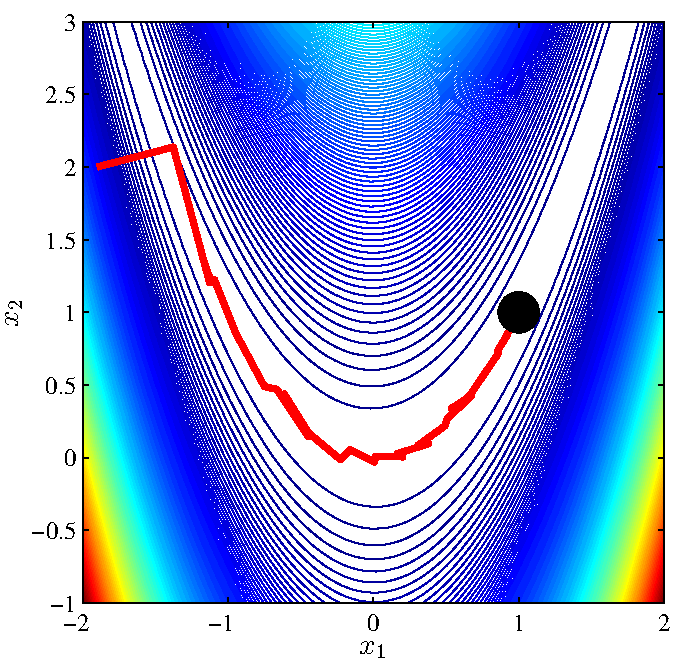
\includegraphics[width=2.8in]{\figurepath/part1_rosen_state.pdf}
    \caption{Search history\label{fig:part1_rosen_state}}
  \end{minipage}
  \hfill
  \begin{minipage}{.48\textwidth}
    \centering
    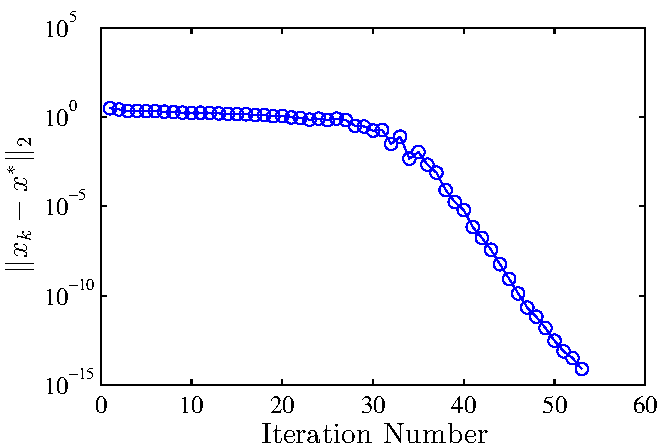
\includegraphics[width=3.2in]{\figurepath/part1_rosen_convergence.pdf}
    \caption{Convergence history\label{fig:part1_rosen_convergence}}
  \end{minipage}
\end{figure}

\clearpage
\subsection*{(2) Second Objective Function}

In this problem, the following objective function was used instead of the Rosenbrock function.

\begin{equation*}
f(x_{1},x_{2})=x_{1}^{4}+100x_{2}^{4}
\end{equation*}

The BFGS code was used, with the appropriate function handle passed to find the minimum.
Figure~\ref{fig:part2_objective2_state} shows the search history plotted in the $x_{1}$, $x_{2}$ plane.
Figure~\ref{fig:part2_objective2_convergence} shows the convergence history, the distance of each point $x_{k}$ in the BFGS iteration from the optimal solution $x^{*}$.
The optimal solution for this objective function can be found by inspection as $x_{1}=0$, $x_{2}=0$ with $f(0,0)=0$.
From Figure~\ref{fig:part2_objective2_convergence} we can see that the convergence is linear.
Additionally, this is expected due to the objective function having 4th power.

\begin{figure}[H]
  \centering
  \begin{minipage}{.48\textwidth}
    \centering
    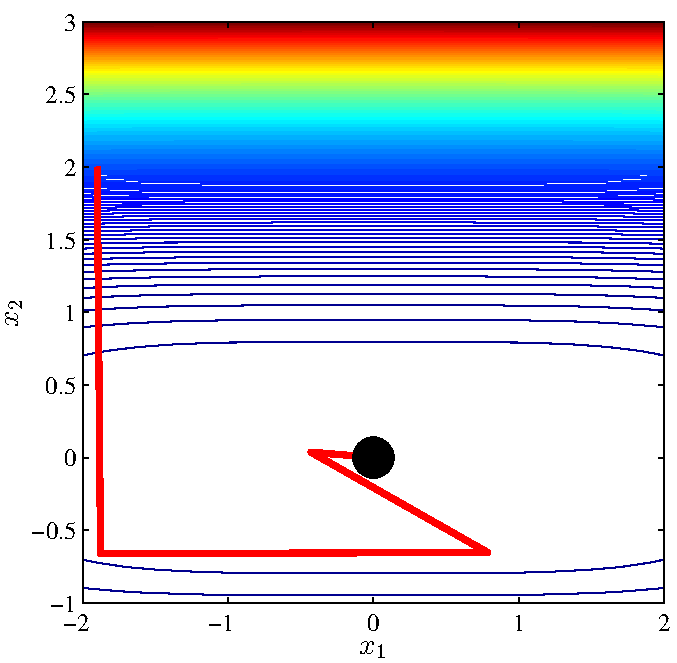
\includegraphics[width=2.7in]{\figurepath/part2_objective_state.pdf}
    \caption{Search history\label{fig:part2_objective2_state}}
  \end{minipage}
  \hfill
  \begin{minipage}{.48\textwidth}
    \centering
    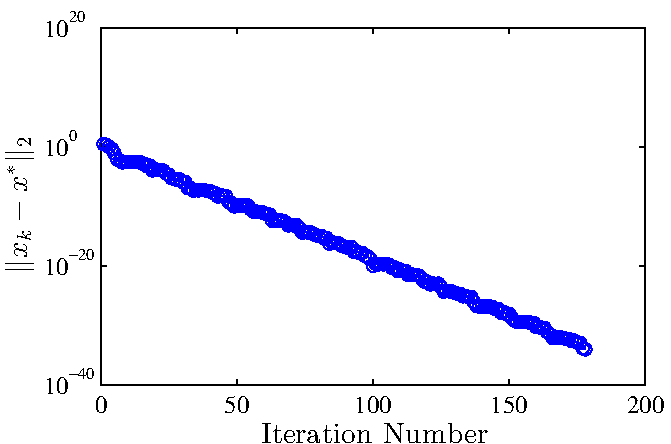
\includegraphics[width=3.3in]{\figurepath/part2_objective2_convergence.pdf}
    \caption{Search history\label{fig:part2_objective2_convergence}}
  \end{minipage}
\end{figure}

\clearpage
\subsection*{(3) Multiple Minima}

For the following function

\begin{equation*}
f(x_{1},x_{2})=2x_{1}^{2}-1.05x_{1}^{4}+\frac{1}{6}x_{1}^{6}-x_{1}x_{2}+x_{2}^{2}
\end{equation*}

From Figures~\ref{fig:part3_multiple_state}-\ref{fig:part3_multiple_state_ic3} we can see the presence of three minima in the region $-3\leq x_{1}\leq3$, $-3\leq x_{2}\leq3$.
The minima values are listed in the caption below each figure.
There are two stationary points corresponding to the saddle points which can clearly be seen in Figures~\ref{fig:part3_multiple_state}-\ref{fig:part3_multiple_state_ic3}.
The saddle points are at $(x_{1},x_{2})=(1.0706,0.5353)$ and $(-1.0706,-0.5353)$ as evaluated analytically and solved the roots of a fifth order polynomial using \textsc{Matlab}.

\begin{figure}[H]
  \begin{center}
    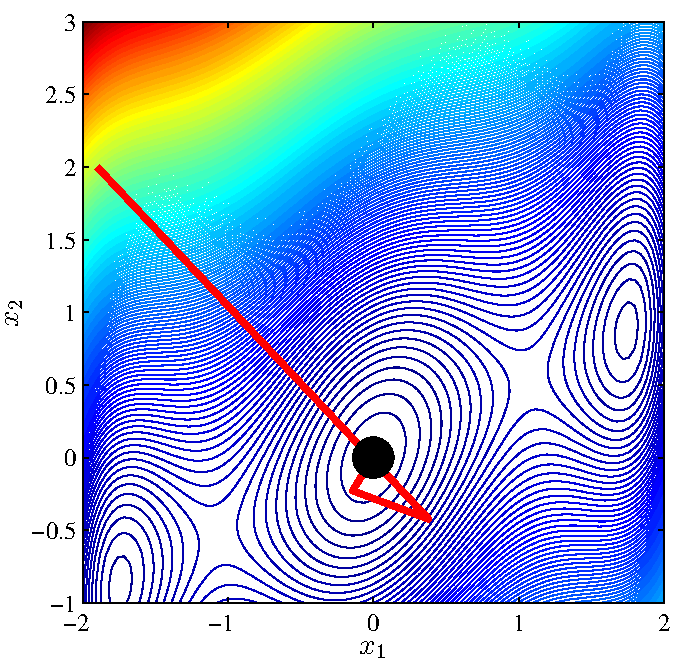
\includegraphics[width=2.6in]{\figurepath/part3_multiple_state.pdf}
    \caption{Search history starting from initial condition of $x_{1}=-1.9$, $x_{2}=2$, converging to the minimum at $x_{1}=0$, $x_{2}=0$ where $f(0,0)=0$.\label{fig:part3_multiple_state}}
  \end{center}
\end{figure}

\vspace{-0.5in}

\begin{figure}[H]
  \centering
  \begin{minipage}{.48\textwidth}
    \centering
    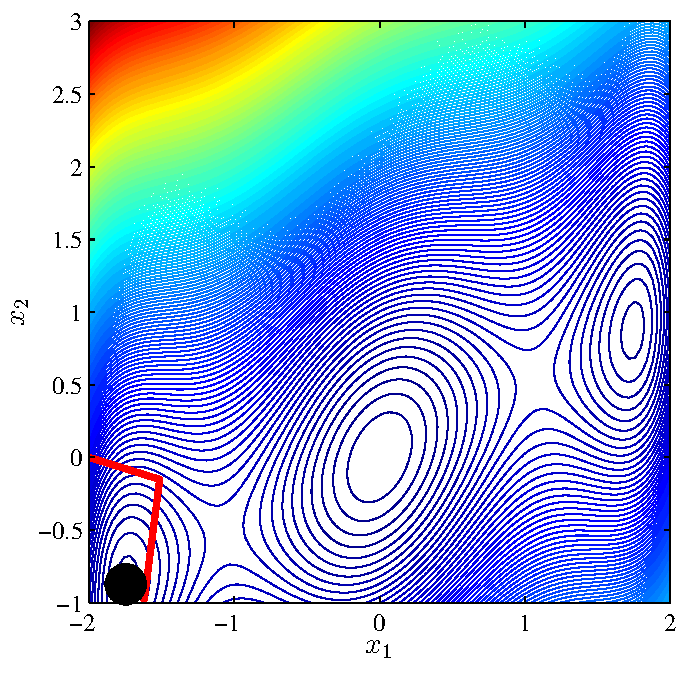
\includegraphics[width=2.6in]{\figurepath/part3_multiple_state_ic2.pdf}
    \caption{Search history starting from initial condition of $x_{1}=-2$, $x_{2}=0$, converging to the minimum at $x_{1}=-1.7476$, $x_{2}=-0.8738$ where $f(-1.7476,-0.8738)=0.2986$.\label{fig:part3_multiple_state_ic2}}
  \end{minipage}
  \hfill
  \begin{minipage}{.48\textwidth}
    \centering
    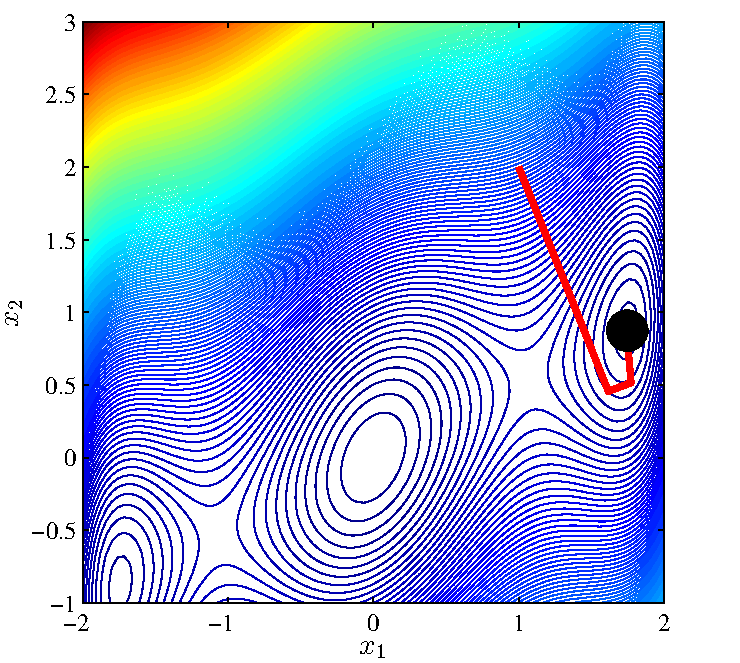
\includegraphics[width=2.8in]{\figurepath/part3_multiple_state_ic3.pdf}
    \caption{Search history starting from initial condition of $x_{1}=1$, $x_{2}=2$, converging to the minimum at $x_{1}=1.7476$, $x_{2}=0.8738$ where $f(1.7476,0.8738)=0.2986$.\label{fig:part3_multiple_state_ic3}}
  \end{minipage}
\end{figure}

\clearpage
\section*{Constrained Minimization}

\subsection*{(4) Rectangle in Ellipse}

For this problem we can solve it two ways.
The first method is substitution, where the equality constraint is used to solve for one variable in terms of the other, and then this is substituted into the objective function.
The objective function then depends on only one variable, and this function can be maximized by differentiating and setting the derivative to zero.
Substitution works well for linear constraints, but is hard to generalize for larger systems and nonlinear constraints.
So, The other way is with Lagrange multipliers.
The problem is

\begin{align*}
  &\text{maximize }\quad P(x,y)=4(x+y) \\
  &\text{subject to }\quad\frac{x^{2}}{a^{2}}+\frac{y^{2}}{b^{2}}=1
\end{align*}

\paragraph{Method 1: Substitution}

Solving for $x$ from the constraint we have

\begin{equation*}
  x=\sqrt{a^{2}\left(1-\frac{y^{2}}{b^{2}}\right)}
\end{equation*}

Plugging this into $P$ we have

\begin{equation*}
  P=4\left[a^{2}\left(1-\frac{y^{2}}{b^{2}}\right)\right]^{\frac{1}{2}}+4y
\end{equation*}

Differentiating

\begin{equation*}
  \frac{dP}{dy}=2\left[a^{2}\left(1-\frac{y^{2}}{b^{2}}\right)\right]^{-\frac{1}{2}}\left(2\frac{a^{2}}{b^{2}}y+4\right)+4
\end{equation*}

$\frac{dP}{dy}=0$ implies

\begin{equation*}
  \boxed{%
  y=\frac{b^{2}}{\sqrt{a^{2}+b^{2}}}
  \qquad\text{and}\qquad
  x=\frac{a^{2}}{\sqrt{a^{2}+b^{2}}}}
\end{equation*}

\paragraph{Method 2: Lagrange Multipliers}

\begin{equation*}
  L(x,y,\lambda)=P(x,y)+\lambda c(x,y)
\end{equation*}

where

\begin{equation*}
  c(x,y)=\frac{x^{2}}{a^{2}}+\frac{y^{2}}{b^{2}}-1=0
\end{equation*}

Evaluate

\begin{align*}
  \frac{\partial L}{\partial x}&=4+\frac{2\lambda}{a^{2}}x=0 \\
  \frac{\partial L}{\partial y}&=4+\frac{2\lambda}{b^{2}}y=0 \\
  \frac{\partial L}{\partial\lambda}&=\frac{x^{2}}{a^{2}}+\frac{y^{2}}{b^{2}}-1=0
\end{align*}

Solving this system of three equations and three unknowns we arrive at the same result as using the substitution method.

\subsection*{(5) Parallelpiped in Ellipsoid}

\begin{align*}
  &\text{maximize }\quad V(x,y,z)=8xyz \\
  &\text{subject to }\quad\frac{x^{2}}{a^{2}}+\frac{y^{2}}{b^{2}}+\frac{z^{2}}{c^{2}}-1=0
\end{align*}

For this problem use Lagrange multipliers

\begin{equation*}
  L(x,y,z,\lambda)=8xyz+\lambda\left(\frac{x^{2}}{a^{2}}+\frac{y^{2}}{b^{2}}+\frac{z^{2}}{c^{2}}-1\right)
\end{equation*}

Evaluate

\begin{align*}
  \frac{\partial L}{\partial x}&=8yz+\frac{2\lambda}{a^{2}}x=0 \\
  \frac{\partial L}{\partial y}&=8xz+\frac{2\lambda}{b^{2}}y=0 \\
  \frac{\partial L}{\partial z}&=8xy+\frac{2\lambda}{c^{2}}z=0 \\
  \frac{\partial L}{\partial\lambda}&=\frac{x^{2}}{a^{2}}+\frac{y^{2}}{b^{2}}+\frac{z^{2}}{c^{2}}-1=0
\end{align*}

Solving the first three equations for $\lambda$ and equating, we have

\begin{equation*}
  -\frac{4yza^{2}}{x}=-\frac{4xzb^{2}}{y}=-\frac{4xyc^{2}}{z}
\end{equation*}

giving

\begin{equation*}
  x^{2}=\frac{a^{2}}{b^{2}}y^{2}
  \qquad
  z^{2}=\frac{c^{2}}{b^{2}}y^{2}
  \qquad
  z^{2}=\frac{c^{2}}{a^{2}}x^{2}
\end{equation*}

Plugging these into the last equation we obtain

\begin{equation*}
  \boxed{%
  x=\frac{a}{\sqrt{3}}
  \qquad\text{and}\qquad
  y=\frac{b}{\sqrt{3}}
  \qquad\text{and}\qquad
  z=\frac{c}{\sqrt{3}}}
\end{equation*}

\clearpage
\section*{(6) Inequality Constraints}

To solve an optimization problem with inequality constraints, we essentially only need to take into account the active constraints.
To do this, we multiply the partial derivatives of the Lagrangian with respect to each multiplier by the corresponding multiplier, as shown below.
We then consider all the different cases where $\lambda_{i}=0$ indicating the constraint is inactive and $\lambda_{j}\neq0$ indicating the constraint is active.
By multiplying by the extra factor of $\lambda$, the equations will still be solvable regardless of whether each $\lambda_{i}$ is zero or not, either because the constraint is inactive, or because the constraint is satisfied.

\begin{align*}
  f(x,y)&=x^{2}+y^{2}-6xy-4x-5y \\
  c_{1}(x,y)&=y+(x-2)^{2}-4\leq0 \\
  c_{2}(x,y)&=1-x-y\leq0
\end{align*}

Form the Lagrangian $L(x,y,\lambda_{1},\lambda_{2})=f(x,y)+\lambda_{1}c_{1}(x,y)-\lambda_{2}c_{2}(x,y)$ giving

\begin{equation*}
  L(x,y,\lambda_{1},\lambda_{2})=x^{2}+y^{2}-6xy-4x-5y+\lambda_{1}\left[y+(x-2)^{2}-4\right]+\lambda_{2}\left[1-x-y\right]
\end{equation*}

Form necessary conditions

\begin{align*}
  \frac{\partial L}{\partial x}&=2x-6y-4+2\lambda_{1}(x-2)-\lambda_{2}=0 \\
  \frac{\partial L}{\partial y}&=2y-6x-5+\lambda_{1}-\lambda_{2}=0 \\
  \lambda_{1}\frac{\partial L}{\partial\lambda_{1}}&=\lambda_{1}\left[y+(x-2)^{2}-4\right]=0 \\
  \lambda_{2}\frac{\partial L}{\partial\lambda_{2}}&=\lambda_{2}(1-x-y)=0
\end{align*}

Now we need to consider the various options in terms of which constraints are active/inactive.

\paragraph{Both constraints inactive: $\boldsymbol{\lambda_{1}=\lambda_{2}=0}$}

Substituting these values of $\lambda$ into the above equations we get

\begin{align*}
  2x-6y-4&=0 \\
  2y-6x-5&=0
\end{align*}

which gives the solution $y=-\frac{17}{16}$, $x=\frac{5}{8}$.
Plugging these values back into the constraints, we can see that the constraints are not satisfied, so this is not a valid option.

\paragraph{Inactive: $\boldsymbol{\lambda_{1}=0}$, active: $\boldsymbol{\lambda_{2}\neq0}$}

Next we try making $\lambda_{2}$ active, giving the following equations.

\begin{align*}
2x-6y-4-\lambda_{2}&=0 \\
2y-6x-5-\lambda_{2}&=0 \\
\lambda_{2}(1-x-y)&=0
\end{align*}
From the third equation we have $x=1-y$ and substituting that into the first two equations we have
\begin{align*}
2(1-y)-6y-4-\lambda_{2}&=0 \\
2y-6(1-y)-5-\lambda_{2}&=0 \\
\end{align*}

which can be solved yielding $y=\frac{9}{16}$, $x=\frac{7}{16}$ and $\lambda_{2}=-\frac{13}{2}$.
Checking the constraints, we can see that they are both satisfied.
So this point is a valid solution, but we aren't yet sure whether this is actually the minimum until we try the other combinations of active and inactive constraints.
Evaluating the function here, we have $f\left(\frac{7}{16},\frac{9}{16}\right)=-5.53$.

\paragraph{Active: $\boldsymbol{\lambda_{1}\neq0}$, inactive: $\boldsymbol{\lambda_{2}=0}$}

\begin{align*}
2x-6y-4+2\lambda_{1}(x-2)&=0 \\
2y-6x-5+\lambda_{1}&=0 \\
\lambda_{1}\left[y+(x-2)^{2}-4\right]&=0
\end{align*}

From the third equation we can solve $y=4-(x-2)^{2}$ and plug into the first two giving

\begin{align*}
  2x-6\left[4-(x-2)^{2}\right]-4+2\lambda_{1}(x-2)&=0 \\
  2\left[4-(x-2)^{2}\right]-6x-5+\lambda_{1}&=0
\end{align*}

From the second equation solve for $\lambda_{1}$ as

\begin{equation*}
  \lambda_{1}=6x+5-2\left[4-(x-2)^{2}\right]
\end{equation*}

Then substitute this into the first equation

\begin{equation*}
  2x-6\left[4-(x-2)^{2}\right]-4+2\left(6x+5-2\left[4-(x-2)^{2}\right]\right)(x-2)=0
\end{equation*}

and simplify

\begin{align*}
  2x-6\left[4-(x-2)^{2}\right]-4+2\left(6x+5-2\left[4-(x-2)^{2}\right]\right)(x-2)&=0 \\
  2x-6\left[4-x^{2}+4x-4\right]-4+2\left(6x+5-8+2x^{2}-8x+8\right)(x-2)&=0 \\
  2x+6x^{2}-24x-4+(-4x+10+4x^{2})(x-2)&=0 \\
  6x^{2}-22x-4-4x^{2}+10x+4x^{3}+8x-20-8x^{2}&=0 \\
  4x^{3}-6x^{2}-4x-24&=0
\end{align*}

Solving this equation numerically we have $x=2.6962$, $y=3.5153$, $f(2.6962,3.5153)=-65.6023$ and $\lambda_{1}=14.1469$.

\paragraph{Both active: $\boldsymbol{\lambda_{1}\neq0}$, $\boldsymbol{\lambda_{2}\neq0}$}

In this case we use the fourth and fifth equations to find the equation $x^{2}-5x+1=0$, and $y=1-x$.
Solving these equations we get four different possible solutions, none of which is a minimum.

\subsection*{Minimum}

After checking all of the cases for the constraints being active or inactive, we found the minimum is given by the following

\begin{equation*}
  \addtolength{\fboxsep}{5pt}
  \boxed{%
  \begin{split}
    x&=2.6962 \\
    y&=3.5153 \\
    f&=-65.6023 \\
    \lambda_{1}&=14.1469
  \end{split}}
\end{equation*}

\subsection*{Sensitivity}

At the minimum found above, we can rewrite the constraint $c_{1}(x,y)\leq0$ as $\bar{c}_{1}(x,y)\leq C$ where $C=4$.
If $C$ is changed, the change in the minimum is given by $\frac{\partial f}{\partial C}=-\lambda_{1}$.
So, if $C=4.1$ then we have $\frac{\partial f}{\partial C}=-14.1469$.
To compute the total change we compute

\begin{align*}
  \Delta f&=\frac{\partial f}{\partial c_{1}}\Delta c_{1} \\
  &=-\lambda_{1}\Delta c_{1} \\
  &=-14.1469(0.1) \\
  &-1.41469
\end{align*}

So, if the cost function is changed as shown, then the minimum that can be achieved becomes smaller.
So the new minimum would be

\begin{equation*}
  \boxed{%
  f(x,y)=-67.02}
\end{equation*}

\subsection*{Writing a Script to Confirm Results}

A script was written which uses the \textsc{Matlab} function \texttt{fmincon.m} to solve the constrained minimization, yielding the same results as determined above.
The code can be found in the appendix.

\section*{(7) Bryson Paper Summary}

The calculus of variations is the foundation upon which optimal control theory was built.
The calculus of variations deals with optimizing a function $J(y)$ over the set of admissible functions $y(x)$.
The calculus of variations started with Pierre de Fermat.
Galileo Galilei posed two problems which were later solved using CV.%
John Bernoulli and Leibniz used Fermat's ideas to solve one of Galileo's problems.
Isaac Newton is credited with inventing CV in 1685.
Leonard Euler provided the beginnings of a real theory of CV, and Lagrange invented the method of Lagrange multipliers that we use today.
During the early to mid 1800s, Gustav Jacob Jacobi and William Rowan Hamilton were working on what would later become the Hamilton-Jacobi-Bellman equation, developed by Bellman in the mid 1900s.
Also during the mid 1800s, Karl Wilhelm Theodor Weierstrass was also working on CV on a more rigorous basis, on which Bellman and Pontryagin built in the 1900s.

In 1960s, this theory had led to optimal control as it is known at the undergraduate level today.
Kalman used a quadratic function to penalize state variables and control inputs, and used CV to derive an optimal control law which turned out to be linear constant gain feedback of the state variables, which was later renamed by Athans as LQR control.
Furthermore, this idea was extended to the estimator problem, giving rise to the LQE, where the expected value of the integral quadratic performance index in the presence of Gaussian white noise.
Combining LQE and LQR resulted in the LQG compensator, which is widely used today.
Also around this time nonlinear programming was also being developed, whose successful application was crucially dependent on the invention of the digital computer.
Dynamic programming was an extension of the work of Hamilton and Jacobi, also being developed in the 1950s, and the Euler-Lagrange equations of CV can also be derived using dynamic programming.

This theory was finally able to be applied to practical applications using numerical solutions and the computer, such as optimal trajectory generation for fighter jets, as well as for developing logic used in the Apollo 11 moon landing in 1969.
Much work at this time by people such as Bryson and Ross was done to develop numerical algorithms.
Also at this time, Kalman and McFarlane were some of the people working with Riccati equations to solve the LQ optimal control problem, resulting in the elegant, efficient method we know today.
During the 1970s much focus was turned toward robustification of the optimal control methods, and development of $H_{\infty}$ control theory.

\clearpage
\section*{Code}

\lstinputlisting{\codepath/master_hw1_v2.m}
\lstinputlisting{\codepath/bfgs.m}
\lstinputlisting{\codepath/linesearch.m}
\lstinputlisting{\codepath/functionpart1_rosen.m}
\lstinputlisting{\codepath/functionpart2_objective.m}
\lstinputlisting{\codepath/functionpart3_multiple.m}
\lstinputlisting{\codepath/problem6_master.m}
\lstinputlisting{\codepath/problem6_function.m}
\lstinputlisting{\codepath/problem6_constraints.m}

\end{document}
